SE and opinion mining is the field of study that analyzes people's opinions, sentiments, evaluations, attitudes, and emotions from written language.\cite{liu2012sentiment} It's also known as emotion AI or opinion mining. The main and basic task of this field is to correctly classify the polarity of a particular text and evaluate whether is it positive, negative or in some cases neutral. It can be used in almost any situation where data need to be analysed for its sentiment aspect, what means the application options are almost endless.  for example product reviews, online discussions or social media content.

SE is in demand mostly because of its efficiency. Tens of thousands of documents can be analysed within seconds and despite results are not always as exact as human workers would produce, the efficiency boost is often too big not to take advantage of it.

SE can be divided into several steps:
\begin{enumerate}
  \item \textbf{Data collection} - involves all the substeps required to gather user-generated content from any source. Surveys, blogs, various forums and social media. These all contains huge amount of real people from real world with real experiences. These data are always expressed completely different - using slang, shortcuts, internet language or generally just being used in different context.
  \item \textbf{Data preprocessing} - this step represents cleaning the data. Data preprocessing can often have a significant impact on generalization performance of a supervised ML algorithms \cite{kotsiantis2006data} and if there is much irrelevant information and data are unreliable, then knowledge discovery during the training phase is more difficult. It removes irrelevant content which could potentially lead to bad and incorrect results. This is a very delicate step because it manipulates the raw data and if not done correctly, it can easily change results.
  \item \textbf{Sentiment detection} - this step basically stands for training of the classifier. Subjective feelings and expressions are highlighted, emphasized and retained while objective information like facts are discarded and ignored. 
  \item \textbf{Sentiment classification} - subjective expressions are classified.
    \item \textbf{Output interpretation} - graphical presentation of obtained results. Time and sentiment can be analyzed to construct various charts, graphs, timelines and many other metrices.
\end{enumerate}

\subsubsection{History}
Interest in opinion of other individuals is probably as old as the communication itself. There is evidence that already in ancient Greece, generals were trying to detect dissent among their subordinates using various "primitive" approaches \cite{richmond1998spies}. Another approach to measure and evaluate a public opinion coming from ancient Greece and used to these date is voting. In the first decades of twentieth century, efforts in capturing public opinion started utilize questionaires and in 1937, first scientific journal on public opinion was founded. 

In the last 10 years, SE and ML in general experienced a big boom. According to data collected by Mantyla, Graziotin and Kuutila \cite{mantyla2018evolution}, nearly 7000 papers about sentiment analysis have already been written and not surprisingly, 99\% of them were published after 2004 - making sentiment analysis one of the fastest growing research areas. The increasing interest about this area as published by Mantyla, Graziotin and Kuutila \cite{mantyla2018evolution} can be seen in the graph \ref{fig:papersCountHistory}.

\begin{figure}[H]%
    \centering
	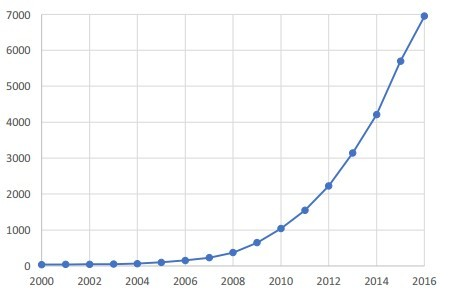
\includegraphics[width=8cm]{papersCountHistory.jpg}
    \caption{Cumulative count of papers about sentiment analysis}%
    \label{fig:papersCountHistory}%
\end{figure}



\subsubsection{Training datasets}
One of the main building blocks of any correctly and accurately functioning ML projects is a training phase. It can actually be seen as a base for the whole project. One can have the best fine-tuned optimized classifier, but if the training data he used do not fit the domain where the classifier is intended to be used, results of the classifier can be (surprisingly) bad. It's the same as house and its base. If the base is not done correctly, however cool architectural solution have other storeys used, house is still going to fall in the next big storm.

That's why choosing a sufficient and fitting dataset to train my classifiers was a very important task. The datasets I've considered were:
\begin{itemize}
  \item \textbf{Dataset140}\footnote{http://cs.stanford.edu/people/alecmgo/trainingandtestdata.zip} - it is currently the biggest dataset with tweets labeled by their sentiment. What is interesting and makes the dataset special is that opposed to other datasets being manually annotated by humans, this one was created by a program. It contains 1.6 million tweets with their polarity score (0 = negative, 2 = neutral, 4 = positive), tweet id, date of tweet publication, author of the tweet and the text of the tweet. More about how this dataset was created can be found in Go et al. paper \cite{go2009twitter}
  \item \textbf{Movie review data}\footnote{http://www.cs.cornell.edu/people/pabo/movie-review-data/} - Thousand positive and thousand negative labeled movie reviews. This dataset was introduced in Pang/Lee ACL 2004 \cite{pang2004sentimental}
  \item \textbf{Hu-Liu lexicon}\footnote{https://github.com/woodrad/Twitter-Sentiment-Mining/tree/master/Hu\%20and\%20Liu\%20Sentiment\%20Lexicon} - plain list of 6800 common English words labeled as positive and negative
  \item \textbf{Warriner et al lexicon}\footnote{http://crr.ugent.be/archives/1003} - This list of words was collected with Amazon Mechanical Turk. Three components of emotions are distinguished: valence (the pleasantness of a stimulus), arousal (the intensity of emotion provoked by a stimulus), and dominance (the degree of control exerted by a stimulus) \cite{warriner2013norms}. Warriner and Kuperman extended ANEW norms collected by Bradley and Lang from 1034 words to 13,915 words (lemmas).
  \item \textbf{Stack overflow dataset}\footnote{https://sentiment-se.github.io/replication.zip} - Later into the thesis I've decided to test dataset of 1500 manually labeled Stack overflow sentences created by Bin Lin et al. in their late paper on negative results in SA called "How far can we go".
    \item \textbf{My own cryptocurrency tweets dataset} - As already said before, performance of the classifier depends on how close the training data are to the real use-case data. That's why I considered and even started to create my own dataset targeting specifically only cryptocurrency tweets, which I've intended to analyze as well.
\end{itemize}

Big surprise here was the lack of any bigger Reddit dataset.

\subsubsection{Language processing tools}
From the very beginning, I knew I wanted to use Python. I had some slight background knowledge in ML from online courses and most of them were done in Python. Therefore while searching and deciding which library should I use, I've always given a slight edge to the Python options. I've considered (and tested) these:
\begin{itemize}
\item \textbf{NLTK} - probably the best-known Python module for NLP. It provides easy-to-use interfaces for more than 50 corpora and lexical resources. It also offeres a rich palette of processing libraries for classification, tokenization, stemming, tagging, parsing, and semantic reasoning.
\item \textbf{Textblob: Simplified Text Processing} - as a name says, Textblob provides easy processing and is actually built on top of NLTK. It provides a simple API for diving into common natural language processing tasks such as part-of-speech tagging, noun phrase extraction, sentiment analysis (Naive Bayes, Decision Tree), classification, translation and more.
\item \textbf{Scikit-learn} - Python module for general ML, data mining and data analysis. It is built on NumPy, SciPy and matplotlib modules.
\end{itemize}

Also, sentiment analysis is just one part of the task. To evaluate the data and find pattern, basic data science algorithms will be needed. With data science, R is very often listed as a default choice. Therefore were the results of google trends query shown in Figure  pretty surprising. This definitely helped my decision with sticking to Python.

\begin{figure}[H]%
    \centering
	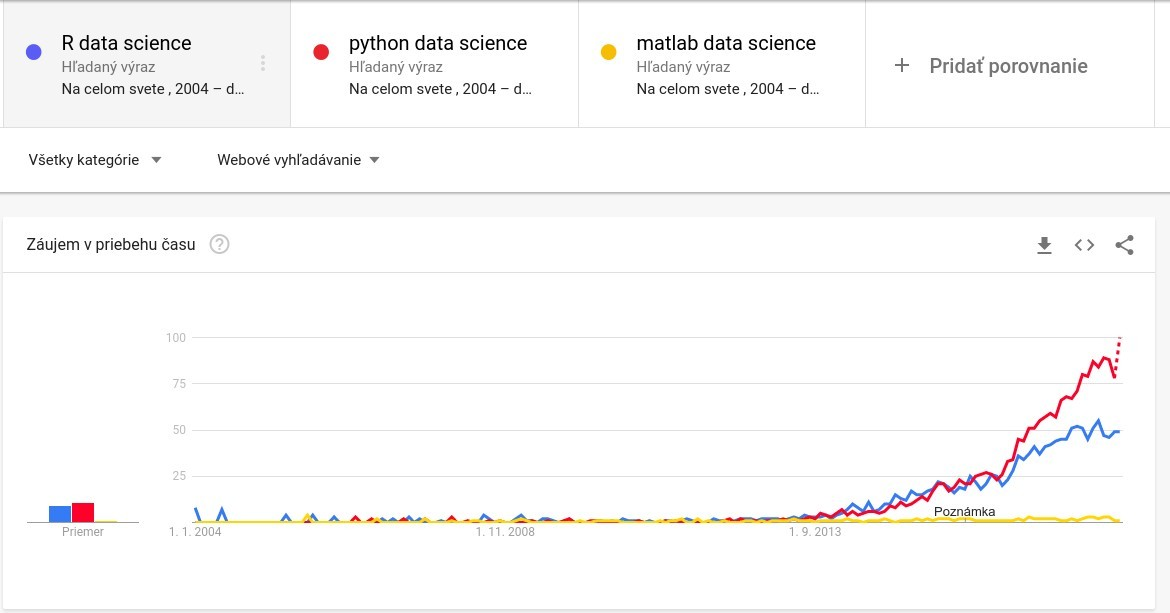
\includegraphics[width=10cm]{PythonMatlabR.jpg}
    \caption{Google trend of searches regarding data science with various programming languages}%
    \label{fig:PythonMatlabR}%
\end{figure}


\subsubsection{Performance metrics}
\paragraph{Terminology} Before diving into talk about the metrics, there are 4 crucial terms which need to be explained:
\begin{itemize}
\item \textbf{Tue Positives (TP)} - instances correctly labeled as positive
\item \textbf{True Negatives (TN)}- instances correctly labeled as negative
\item \textbf{False Positives (FP)} - instances incorrectly labeled as positive
\item \textbf{False Negatives (FN)}- instances incorrectly labeled as negative
\end{itemize}


The metrics that you choose to evaluate your machine learning algorithms are very important and not all are suitable for every situation. Choice of metrics influences how the performance of machine learning algorithms is measured and choosing a wrong evaluation metric for particular use could potentially lead towards eliminating the best performing algorithm in favour of the worse one.
Here are some of the most often used metrics used to evaluate classification algorithms. It's also useful to choose the metric before doing the analysis, so you won't get distracted by already having the results in case of doing the decision later.

\begin{itemize}
\item \textbf{Classification accuracy} - this is the most intuitive and common evaluation metric for classification problems but it is also the most misused one. It is really only suitable when there are an equal number of observations in each class (which is rarely the case) and that all predictions and prediction errors are equally important, which is often not the case. In case of imbalanced dataset with 9\% of instances in one class and only 10\% in the other, predicting every instance as a majority class without even considering its features would lead to high accuracy of 90\%. This is called \textbf{accuracy paradox.}
\[ Accuracy = \frac{TP + TN}{TP + TN + FP + FN}\]
\item \textbf{Confusion matrix} - clean and unambiguous way to present the prediction results of a classifier. If the classification is binary (there are only 2 classes), this matrix has 2 rows and 2 columns - therefore altogether 4 cells which are filled with true/false positives/negatives count. Such scenario is demonstrated in table \ref{table:Confusion_matrix_general}. Although the confusion matrix shows all of the information about the classifier's performance, more meaningful measures can be extracted from it to illustrate certain performance criteria.\cite{bradley1997use}. 
\begin{table}[H]
{
\centering
\begin{tabular}{ |p{4cm}|p{4cm}|p{4cm}|  }
 \hline
 \multicolumn{3}{|c|}{Confusion matrix} \\
 \hline
  & Predicted positive & Predicted negative\\
 \hline
 Real positive   & TP    &FN\\ \hline
 Real negative &   FP  & TN\\ \hline
\end{tabular}
}
\caption{Confusion matrix}
\label{table:Confusion_matrix_general}
\end{table}

\item \textbf{Precision} - Precision can be seen as a representation of a classifiers exactness. A low precision can also indicate a large number of False Positives. If the precision is high, it says that there's a high probability of positive label being True Positive. It cannot be tricked but it also hides a lot.
\[ Precision = \frac{TP}{TP + FP}\]
\item \textbf{Recall} - also called \textit{sensitivity} or the \textit{True Positive Rate}, it is a number of True Positives divided by the number of True Positives and the number of False Negatives. In other words, it is a ratio of how many of all positive instances have been identified. Recall can be tricked (labeling all as majority class) but if used next to precision, it gives extra information
\[ Recall = \frac{TP}{TP + FN}\]
\item \textbf{F measure} - as already mentioned, precision hides some facts and recall can be tricked. To give the full story, they need to be used together. That's what F measure is for.
\[ F = 2 * \frac{precision * recall}{precision + recall}\]
\end{itemize}Nice example to demonstrate difference between precision and recall is the concept of Indian Jurisprudence, where "100 culprits may let go free but no innocent should be punished". If we let go so many culprits in order to ensure no innocent is punished, recall will be pretty low, but precision very high.


\subsubsection{Cross-correlation between releases and sentiment change}
When working with time series, we often want to determine whether one series causes changes in another. To find this relationship, measuring a cross-correlation and finding a lag is one way how to do it. Lag represents when change in one data series transfers to the other several periods later. 

To ensure a cross-correlation calculation makes sense, first I have to determine, whether are the data stationary. A stationary time series is one whose properties do not depend on the time at which the series is observed\cite{hyndman5forecast}. More precisely, if y\textsubscript{t} is a stationary time series, then for all \textit{s}, the distribution of \textit{(y\textsubscript{t},…,y\textsubscript{t+s})} does not depend on \textit{t}.

To determine whether my data are stationary, I've used the Dickey-Fuller test method of tseries package in R. Results can be seen in the table \ref{table:stationarity_table_sentiment} and \ref{table:stationarity_table_release_count} 

\begin{table}[H]
\centering
\begin{tabular}{ |p{3cm}||p{3cm}|p{3cm}|  }
 \hline
 \multicolumn{3}{|c|}{Stationarity test of web frameworks sentiment data} \\
 \hline
 Framework & Dickey-Fuller & p-value\\
 \hline
 NodeJS   & -2.6775    &0.2964\\ \hline
 AngularJS &   -3.883  & 0.0199\\ \hline
 EmberJS & -4.0783 & 0.0199\\ \hline
 VueJS    &-3.438 & 0.0646\\ \hline
 CakePHP&   -3.480  & 0.04847\\ \hline
 Laravel& -2.57  & 0.3431\\ \hline
 Symfony& -4.3979  & 0.01\\ \hline
\end{tabular}
\caption{Stationarity test of sentiment}
\label{table:stationarity_table_sentiment}
\end{table}

\begin{table}[H]
\centering
\begin{tabular}{ |p{3cm}||p{3cm}|p{3cm}|  }
 \hline
 \multicolumn{3}{|c|}{Stationarity test of web frameworks release count} \\
 \hline
 Framework & Dickey-Fuller & p-value\\
 \hline
 NodeJS   & -2.896    &0.205\\ \hline
 AngularJS &   -2.547  & 0.353\\ \hline
 EmberJS & -3.297 & 0.0802\\ \hline
 VueJS    &-2.158 & 0.511\\ \hline
 CakePHP&   -3.224  & 0.08915\\ \hline
 Laravel& -2.368  & 0.425\\ \hline
 Symfony& -2.218  & 0.488\\ \hline
\end{tabular}
\caption{Stationarity test of release counts}
\label{table:stationarity_table_release_count}
\end{table}

As we can see, p-values are always higher than 0.05 what indicates non-stationarity of the data, therefore I can't calculate the cross-correlation on them in this state. To transform non-stationary data into stationary, 2 approaches can be used. These are differencing and transforming.  I've taken data series and differenced the values in listing \ref{lst:differencing}. I've executed both, seasonal differencing and stationary differencing although seasonal probably was not needed because the data should not be dependant on the season.

\begin{lstlisting}[caption={Used differencing method in R},label={lst:differencing},language=R]
Differencing <- function(x,y)
{
 framework_x_seasdiff <- diff(x,differences=1)  # seasonal differencing
 framework_x_Stationary <- diff(framework_x_seasdiff, differences= 1)
 framework_y_seasdiff <- diff(y, differences=1)
 framework_y_Stationary <- diff(framework_y_seasdiff, differences= 1)
 return(list(framework_x_Stationary,framework_y_Stationary))
}
\end{lstlisting}
New differenced values do appear to be stationary in mean and variance, as the level and the variance of the series stays roughly constant over time. Sentiment for NodeJS before and after differencing can be seen in Figure \ref{fig:NodeJS_Sentiment_before_after}

\begin{figure}[H]%
    \centering
    \subfloat[Before differencing]{{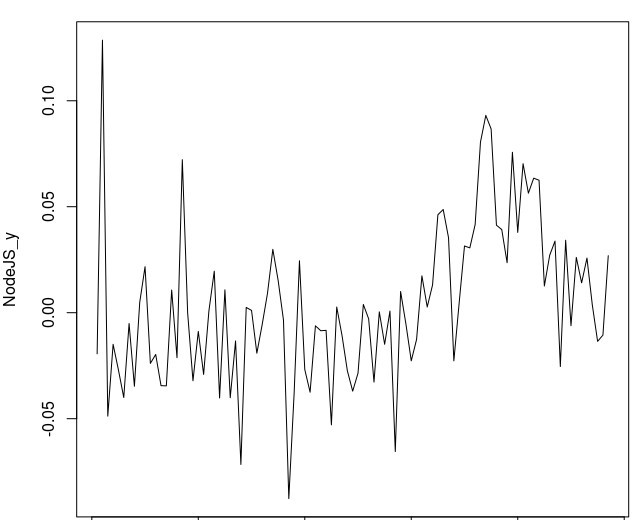
\includegraphics[width=6cm]{NodeJS_before.jpg} }}%
    \qquad
    \subfloat[After differencing]{{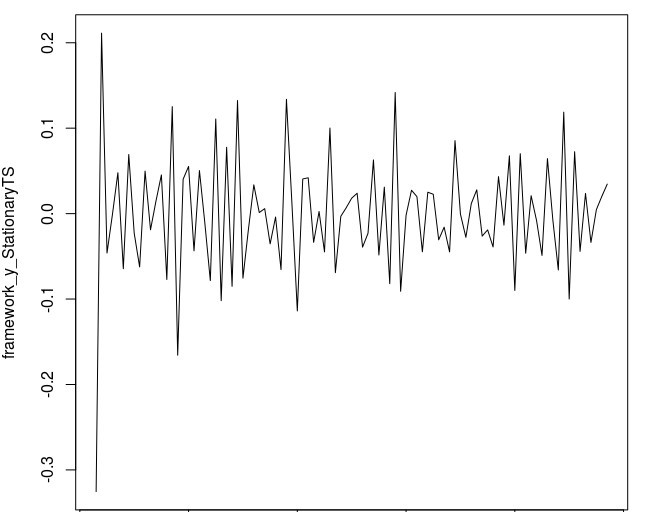
\includegraphics[width=6cm]{NodeJS_after.jpg} }}%
    \caption{NodeJS monthly sentiment values}%
    \label{fig:NodeJS_Sentiment_before_after}%
\end{figure}

Same procedure needed to be done with the "number of releases per month" data and afterwards. Then, cross-correlation could be executed. For this task I've used ccf method in R which implements Pearson's correlation calculation method. Results for all 7 OSS projects can be seen in Figure \ref{fig:highestCorrelationsPlotReleases}

\begin{figure}[H]%
    \centering
	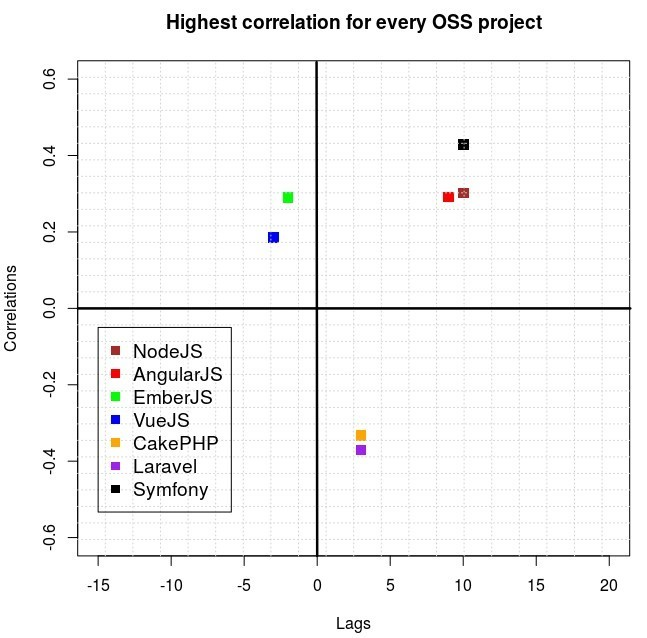
\includegraphics[width=8cm]{highestCorrelationsPlotReleases.jpg}
    \caption{Highest correlations for every OSS project}%
    \label{fig:highestCorrelationsPlotReleases}%
\end{figure}

\paragraph{Results interpretation:}

As we can there is no general pattern. Maximal project correlations happen to occupy 3 of 4 possible quadrants. Each quadrant represents a different relationship between number of releases and sentiment change.

\begin{itemize}
  \item \textbf{I. Quadrant}(Positive correlation + positive lag) - Increase of release count increases a sentiment
  \item \textbf{II. Quadrant}(Positive correlation + negative lag) - Increase of sentiment increases a release count
  \item \textbf{III. Quadrant}(Negative correlation + positive lag) - Increase of release count decreases a sentiment
  \item \textbf{IV. Quadrant}(Negative correlation + Negative lag) - Increase of sentiment decreases a release count
\end{itemize}

Also, in Figure \ref{fig:highestCorrelationsPlotReleases_nonStat} are the results without making the data series stationary. It's obvious that making the data stationary has a big impact on the results.

\begin{figure}[H]%
    \centering
	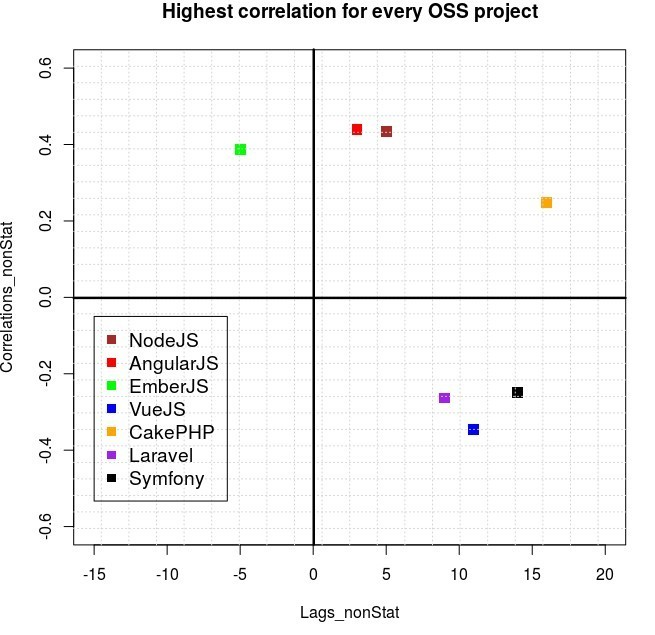
\includegraphics[width=8cm]{highestCorrelationsPlotReleases_nonStat.jpg}
    \caption{Highest correlations for every OSS project (non-stationary)}%
    \label{fig:highestCorrelationsPlotReleases_nonStat}%
\end{figure}

\subsubsection{Commits count within releases}
Initially, I thought that to modify project to take into account a size of the release (amount of commits) will be pretty straightforward task. It actually was straightforward, but as always I've encountered several unexpected problems on the way. \\
I intended to extend my previously used method from Section \ref{ssec:gitReleaseDatesMining} which uses Git API tags endpoint to get the release dates. Unfortunately I wasn't able to find number of commits in the returned objects. JSON object returned from API has following structure:
\begin{lstlisting}
  {
    "url": X,
    "assets_url": X,
    "upload_url": X,
    "html_url": X,
    "id": X,
    "tag_name": X,
    "target_commitish":X,
    "name": X,
    "draft": X,
    "author":{},
    "prerelease": X,
    "created_at": X,
    "published_at": X,
    "assets":[],
    "tarball_url": X,
    "zipball_url":X, 
    }
\end{lstlisting}
I have done some extra searching but did not want to spend extra time so I decided to go the way I knew will work. Instead of using API to get the commit counts, I crawled GitHub UI page of each release and extracted information directly from page source code. Each release details page provides information how many commits behind the current HEAD the commit is. The difference in this number between two following releases represents count of new commits for a release. Results of simple tabular substraction with spreadsheet formula needed to be manually corrected because projects often release several branches parallel and therefore substraction from the previous release was not always the correct one.\\
\\
Eventually, I got correct number of commits for every release and could execute the same cross-correlation analysis described in the previous chapter, but this time instead of releases count, I have explored relationship between sentiment and commits count. One possible flaw in the commit count data are the pre-releases. I treated them as normal releases because they do offer new features but those very same commits are then counted in the official releases later on.\\
\\
After getting the data ready I performed a stationarity test for commit counts. Sentiment values are the same as before with count of releases. Table \ref{table:stationarity_table_commits} shows the results.

\begin{table}[H]
\centering
\begin{tabular}{ |p{3cm}||p{3cm}|p{3cm}|  }
 \hline
 \multicolumn{3}{|c|}{Stationarity test of web frameworks commit counts} \\
 \hline
 Framework & Dickey-Fuller & p-value\\
 \hline
 NodeJS   & -7.0239    &0.01\\ \hline
 AngularJS &   -2.547  & 0.3531\\ \hline
 EmberJS & -3.2764 & 0.0831\\ \hline
 VueJS    &-2.9748 & 0.1886\\ \hline
 CakePHP&   -3.655  & 0.03283\\ \hline
 Laravel& -2.919  & 0.2084\\ \hline
 Symfony& -4.8461  & 0.01\\ \hline
\end{tabular}
\caption{Stationarity test of commit counts}
\label{table:stationarity_table_commits}
\end{table}

I see that there are again several data series (AngularJS, EmberJS, VueJS, Laravel + NodeJS because of unstationarity of sentiment data) which are not stationary so exactly as before with release counts, I had to transform the data. After that, Pearson's cross correlation was calculated. Results for all 7 OSS projects can be seen in Figure \ref{fig:highestCorrelationsPlot}

\begin{figure}[H]%
    \centering
	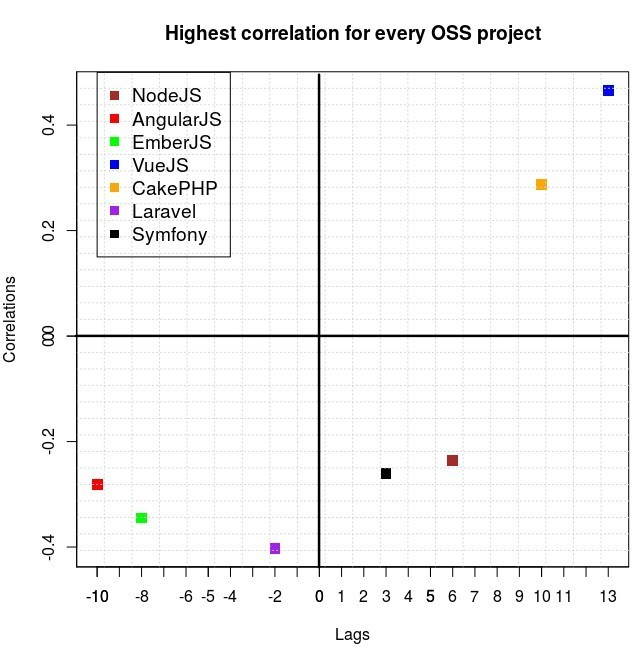
\includegraphics[width=8cm]{highestCorrelationsPlot.jpg}
    \caption{Highest correlations for every OSS project}%
    \label{fig:highestCorrelationsPlot}%
\end{figure}

If I would skip the step of making the data stationary, results would again look completely different \ref{fig:highestCorrelationsPlot_nonStat}.

\begin{figure}[H]%
    \centering
	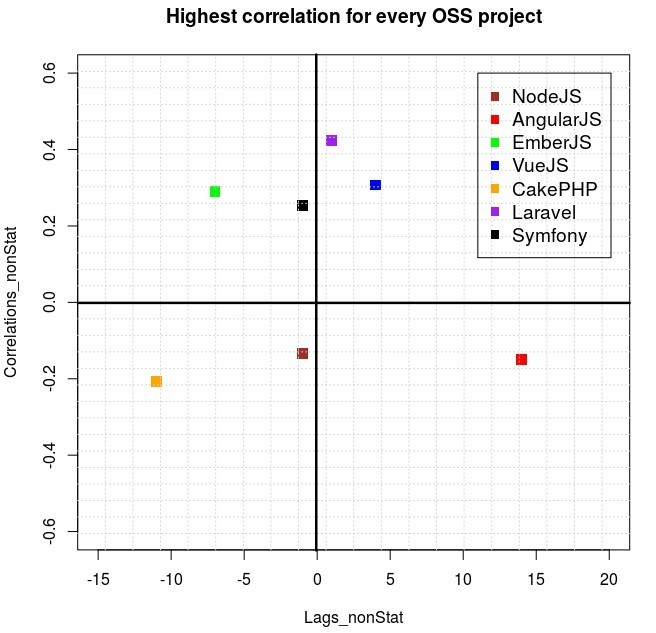
\includegraphics[width=8cm]{highestCorrelationsPlot_nonStat.jpg}
    \caption{Highest correlations for every OSS project (non-stationary)}%
    \label{fig:highestCorrelationsPlot_nonStat}%
\end{figure}
